% generated by scripts/pkl_to_latex.py
% source PKL : vscan_v1_L8_Ne8_U10_t1_mode-uniform_nmin2_solver-gcg_full_restarts10_iter300_kmax5_tol1em09_V0to12_N25-ebabade1a2a1.pkl
% scan type  : vscan
% state      : gs
% quantity   : vn-entropy
% requires   : \usepackage{pgfplots} \pgfplotsset{compat=1.18}
% colours match the matplotlib PDF (tab10 cycle)
\definecolor{gmeC0}{HTML}{1F77B4}
\definecolor{gmeC1}{HTML}{FF7F0E}
\definecolor{gmeC2}{HTML}{2CA02C}
\definecolor{gmeC3}{HTML}{D62728}
\definecolor{gmeC4}{HTML}{9467BD}
\definecolor{gmeC5}{HTML}{8C564B}
\definecolor{gmeC6}{HTML}{E377C2}
\definecolor{gmeC7}{HTML}{17BECF}

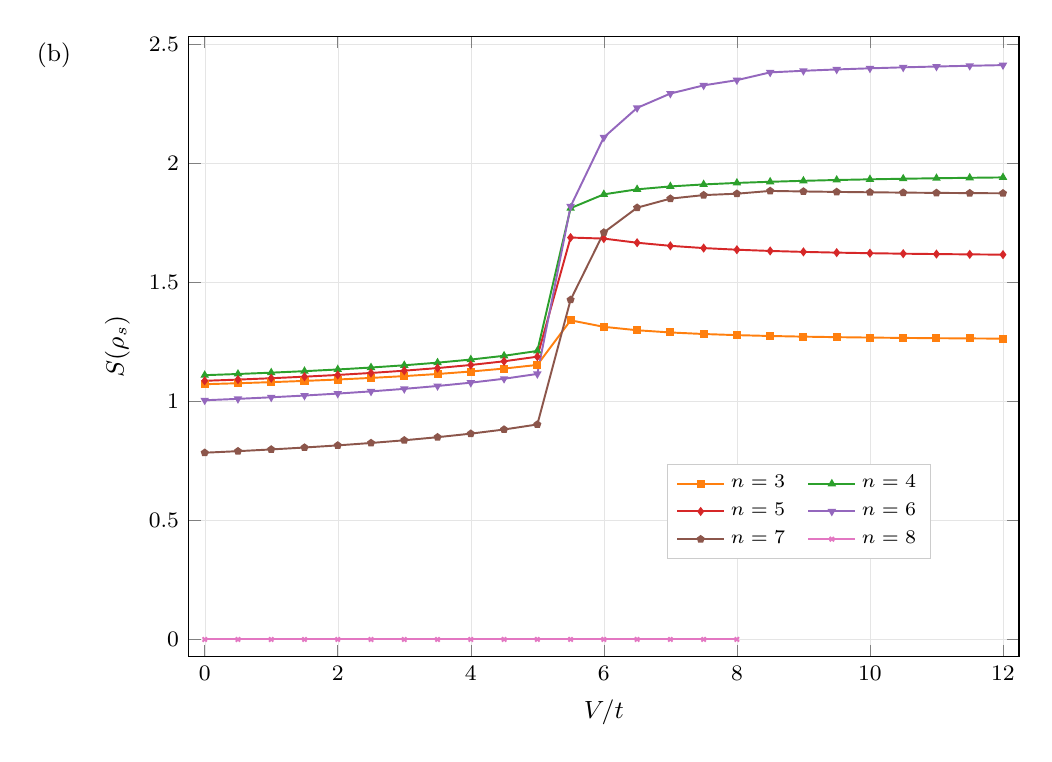
\begin{tikzpicture}
  \begin{axis}[
    width=\columnwidth,
    height=0.78\columnwidth,
    xlabel={$V/t$},
    ylabel={$S(\rho_s)$},
    grid=both,
    grid style={line width=.1pt, draw=gray!20},
    tick label style={font=\footnotesize\rmfamily, /pgf/number format/fixed},
    label style={font=\small\rmfamily},
    scaled ticks=false,
    legend style={font=\scriptsize\rmfamily, draw=gray!40, at={(0.5,1.03)}, anchor=south, /tikz/every even column/.append style={column sep=6pt}},
    legend cell align={left},
    legend columns=2,
    ymin=-0.072,
    ymax=2.532,
    xmin=-0.24,
    xmax=12.24,
    legend style={at={(0.735,0.234)}, anchor=center, fill=white},
    after end axis/.append code={\node[anchor=east, font=\small\rmfamily] at (axis description cs:-0.13,0.970) {(b)};},
  ]
    \addplot[color=gmeC1, mark=square*, mark size=1.1pt, line width=0.7pt] coordinates {
        (0,1.071622) (0.5,1.075706) (1,1.080295) (1.5,1.08547)
        (2,1.091334) (2.5,1.098013) (3,1.105672) (3.5,1.114534)
        (4,1.124916) (4.5,1.137318) (5,1.152628) (5.5,1.339855)
        (6,1.312564) (6.5,1.298191) (7,1.288878) (7.5,1.282387)
        (8,1.277658) (8.5,1.274089) (9,1.271344) (9.5,1.269175)
        (10,1.26743) (10.5,1.266005) (11,1.264826) (11.5,1.263839)
        (12,1.263003)
    };
    \addlegendentry{$n=3$}
    \addplot[color=gmeC2, mark=triangle*, mark size=1.1pt, line width=0.7pt] coordinates {
        (0,1.109563) (0.5,1.114516) (1,1.120086) (1.5,1.126378)
        (2,1.133524) (2.5,1.141694) (3,1.151112) (3.5,1.162095)
        (4,1.175123) (4.5,1.190992) (5,1.211247) (5.5,1.810851)
        (6,1.868869) (6.5,1.889918) (7,1.902069) (7.5,1.910477)
        (8,1.916795) (8.5,1.921577) (9,1.925643) (9.5,1.929023)
        (10,1.931876) (10.5,1.934318) (11,1.936432) (11.5,1.938281)
        (12,1.93991)
    };
    \addlegendentry{$n=4$}
    \addplot[color=gmeC3, mark=diamond*, mark size=1.1pt, line width=0.7pt] coordinates {
        (0,1.085902) (0.5,1.091018) (1,1.096754) (1.5,1.103213)
        (2,1.110521) (2.5,1.118836) (3,1.128367) (3.5,1.139397)
        (4,1.152342) (4.5,1.167869) (5,1.187215) (5.5,1.687419)
        (6,1.682991) (6.5,1.665669) (7,1.65261) (7.5,1.643212)
        (8,1.636332) (8.5,1.631153) (9,1.627209) (9.5,1.624126)
        (10,1.621673) (10.5,1.619692) (11,1.618071) (11.5,1.61673)
        (12,1.615607)
    };
    \addlegendentry{$n=5$}
    \addplot[color=gmeC4, mark=triangle*, mark size=1.1pt, mark options={rotate=180}, line width=0.7pt] coordinates {
        (0,1.004235) (0.5,1.010128) (1,1.016693) (1.5,1.024031)
        (2,1.032267) (2.5,1.041555) (3,1.052091) (3.5,1.064142)
        (4,1.078096) (4.5,1.094579) (5,1.114777) (5.5,1.818104)
        (6,2.108093) (6.5,2.231764) (7,2.292057) (7.5,2.326379)
        (8,2.348317) (8.5,2.380947) (9,2.387652) (9.5,2.393256)
        (10,2.398007) (10.5,2.402085) (11,2.405621) (11.5,2.408718)
        (12,2.41145)
    };
    \addlegendentry{$n=6$}
    \addplot[color=gmeC5, mark=pentagon*, mark size=1.1pt, line width=0.7pt] coordinates {
        (0,0.783959) (0.5,0.79049) (1,0.797729) (1.5,0.80578)
        (2,0.814768) (2.5,0.824848) (3,0.836221) (3.5,0.849152)
        (4,0.864026) (4.5,0.881456) (5,0.902575) (5.5,1.426016)
        (6,1.708757) (6.5,1.812832) (7,1.850856) (7.5,1.865645)
        (8,1.871569) (8.5,1.883218) (9,1.880944) (9.5,1.879047)
        (10,1.877456) (10.5,1.876115) (11,1.874978) (11.5,1.874009)
        (12,1.873178)
    };
    \addlegendentry{$n=7$}
    \addplot[color=gmeC6, mark=x, mark size=1.1pt, line width=0.7pt] coordinates {
        (0,0) (0.5,0) (1,0) (1.5,0)
        (2,0) (2.5,0) (3,0) (3.5,0)
        (4,0) (4.5,0) (5,0) (5.5,0)
        (6,0) (6.5,0) (7,0) (7.5,0)
        (8,0)
    };
    \addlegendentry{$n=8$}
  \end{axis}
\end{tikzpicture}
